\documentclass{article}
\usepackage[utf8]{inputenc}
\usepackage[portuges]{babel}
\usepackage{csquotes}
\usepackage{geometry}
\usepackage[pdftex]{hyperref}
\usepackage{indentfirst}
\usepackage{amsthm}
\usepackage{amssymb}
\usepackage{amsmath}
\usepackage{mathrsfs}
\usepackage{graphicx}
\usepackage{float}
\usepackage{multicol}
\usepackage{verbatim}
\usepackage{dsfont}
\usepackage{pgfplots}
\pgfplotsset{compat = 1.15}

\newtheorem{theorem}{Teorema}
\newtheorem{definition}{Definição}
\newtheorem{lemma}{Lema}
\newtheorem{example}{Exemplo}
\newtheorem{proposition}{Proposição}

\geometry{left = 3cm, top = 3cm, bottom = 2cm, right = 2cm}

\title{Teorema Fundamental das Curvas Espaciais}
\author{Cristhian Grundmann \\ Igor Patrício Michels}
\date{\today}

\begin{document}

\maketitle
\section{Introdução}

No decorrer da primeira parte do semestre foram dadas diversas definições, além de terem sido provadas inúmeras relações, proposições, lemas e teoremas. Tendo em vista isso, nos propomos a provar um teorema não visto em sala, mas que é de extrema importância para o assunto abordado, o Teorema Fundamental das Curvas Espaciais. Tal teorema diz que, dado um intervalo $I =(a, b)\in \mathbb{R}$ e as funções $\kappa : I\to \mathbb{R}^*_+$ e $\tau : I\to \mathbb{R}$, as quais chamaremos de curvatura e torção, respectivamente, definem, a menos de movimentos rígidos, uma curva no espaço.

Esse enunciado, embora simples, é de enorme curiosidade, uma vez que o mesmo não parece nada imediato. Dessa forma, como motivação desse trabalho, vamos buscar entender como uma curva pode ser definida, e construída, a partir de sua curvatura e torção. Algumas demonstrações podem ser vistas em \cite{cruz}-\cite{picado}. Nossa abordagem se dará de forma similar a utilizada por \cite{coda}.

\section{Preliminares}
\label{preliminares}

Primeiramente, é interessante trazer algumas definições de análise que irão nos auxiliar

\begin{definition}(Função Lipschitz-contínua.)
    Seja $M$ um espaço métrico qualquer com a métrica $d$. Uma função $F : M\to M$ é Lipschitz-contínua para todo $x$ e $y$ de $M$ se existe alguma constante $L$ de modo que
    \[d(F(x), F(y))\leq L\cdot d(x, y).\]
    
    O ínfimo das constantes $L$ para os quais vale a desigualdade é chamado de constante de Lipschitz.
\end{definition}

\begin{proposition}
    Se $F$ é uma função Lipschitz-contínua em um intervalo $I$, então $F$ é uma função contínua nesse intervalo.
\end{proposition}

\begin{proof}
    Seja $L$ a constante de Lipschitz de $F$ em $I$. Como $F$ é uma função Lipschitz-contínua, segue da definição que vale
    \[|F(x) - F(y)|\leq L\cdot |x - y|, \forall x, y\in I.\]
    
    Dado $\varepsilon > 0$, considere $\delta = \frac{\varepsilon}{L}$. Dessa forma, $\forall x, y\in I$, de modo que $|x - y| < \delta$, vale que
    \begin{equation*}
        \begin{split}
            |F(x) - F(y)| & \leq L|x - y| \\
            & < L\delta \\
            & = L\cdot \dfrac{\varepsilon}{L} \\
            & = \varepsilon.
        \end{split}
    \end{equation*}
    
    Logo, $F$ é contínua em $I$.
\end{proof}

\begin{lemma}
    \label{lipschitz-continua}
    Se $A$ é uma função continuamente diferenciável e sua derivada é limitada em um intervalo, então $A$ é Lipschitz-contínua no intervalo.
\end{lemma}

\begin{proof}
    Se $A$ possui derivada limitada no intervalo $I$, existe algum $L$ de forma que $|A'(x)|\leq L, \forall x\in I$. Dessa forma, segue pelo Teorema Fundamental do Cálculo, que
    \begin{equation*}
        \begin{split}
            \left|A(x) - A(y)\right| & \leq \left|\int_x^y A'(t) ~dt\right| \\
            & \leq \int_x^y \left|A'(t)\right| ~dt \\
            & \leq L \left|x - y\right|.
        \end{split}
    \end{equation*}
    
    Com resultado seguindo pela definição de Lipschitz-continuidade.
\end{proof}

Feito isso, podemos relembrar o Teorema de Existência e Unicidade de EDO's. Para tanto iremos usar o enunciado de \cite{cruz}.

\begin{theorem}(Existência e Unicidade de Soluções de EDO's.)
    \label{existencia_e_unicidade}
    Considere o problema de valor inicial
    \begin{equation*}
        \begin{split}
            x(0) & = x_0 \\
            x'(t) & = F(x(t)).
        \end{split}
    \end{equation*}
    
    Se $F$ é Lipschitz-contínua em $[0, T]$ então existe uma solução única, $x(t)$ em $C^1(-\infty, \infty)$ com $x(0) = x_0$.
\end{theorem}

\begin{proof}
    Veja o Teorema 5.2 de \cite{cruz}.
\end{proof}

\begin{definition}(Movimento Rígido Positivo.)
    Um movimento rígido positivo é um movimento rígido que preserva a orientação.
\end{definition}

As demais definições e proposições que serão utilizadas já foram trabalhadas em aula, dessa forma optamos por omitir as mesmas. Entretanto, vale lembrar que, assim como \cite{lima}, aqui uma aplicação será dita diferenciável se a mesma for de classe $C^\infty$.

\section{Teorema Fundamental das Curvas Espaciais}

Tendo como base o ferramental apresentado na Seção \ref{preliminares}, podemos enunciar, e provar, o Teorema Fundamental das Curvas Espaciais.

\begin{theorem}(Teorema Fundamental das Curvas Espaciais.)
    \label{teorema_fundamental}
    Sejam $\kappa_0, \tau_0 : I\subseteq \mathbb{R}\to \mathbb{R}$ funções diferenciáveis, com $\kappa_0(t) > 0$. Então existe uma curva $\alpha : I\to \mathbb{R}^3$, parametrizada por comprimento de arco, de modo que $\kappa_\alpha(t) = \kappa_0(t)$ e $\tau_\alpha(t) = \tau_0(t)$.
    
    Além disso, se existe uma outra curva $\beta : I\to \mathbb{R}^3$ de modo que, para todo $t\in I$, seja válido que $\kappa_\beta(t) = \kappa_0(t)$ e $\tau_\beta(t) = \tau_0(t)$, então existe um movimento rígido positivo, $M : \mathbb{R}^3\to \mathbb{R}^3$, tal que $\alpha(t) = M(\beta(t))$.
\end{theorem}

\begin{proof}
    Sejam $T$, $N$ e $B$ os vetores tangente, normal e binormal, respectivamente. Sabemos que os mesmos estão em $\mathbb{R}^3$ e formam o triedro de Frenet, dessa forma, temos que eles respeitam as equações de Frenet-Serret:
    \begin{equation}
        \begin{split}
            T'(t) & = \kappa_0(t) N(t), \\
            N'(t) & = -\kappa_0(t) T(t) + \tau_0(t) B(t), \\
            B'(t) & = -\tau_0(t) N(t).
        \end{split}
        \label{frenet}
    \end{equation}
    
    Note que os vetores $T'(t)$, $N'(t)$ e $B'(t)$ também pertencem ao $\mathbb{R}^3$. Tomando $\gamma : I\to \mathbb{R}^3\times \mathbb{R}^3\times \mathbb{R}^3$ uma curva de modo que
    \[\gamma(t) = \left(T(t), N(t), B(t)\right)\]
    
    \noindent e $F : \mathbb{R}^3\times \mathbb{R}^3\times \mathbb{R}^3\to \mathbb{R}^3\times \mathbb{R}^3\times \mathbb{R}^3$ de tal que
    \[F(\gamma(t)) = \left(\kappa_0(t) N(t), -\kappa_0(t) T(t) + \tau_0(t) B(t), -\tau_0(t) N(t)\right),\]
    
    \noindent temos que $F$ é continuamente diferenciável, logo, pelo Lema \ref{lipschitz-continua}, é Lipschitz-contínua. Agora podemos fixar $t_0\in I$ e considerar a condição inicial de modo que $\gamma(t_0) = \left(e_1, e_2, e_3\right)$, onde $e_i$ são vetores da base canônica. Dessa forma, o Teorema \ref{existencia_e_unicidade} nos garante que existe uma única solução para $\gamma(t)$ de modo que $\gamma'(t) = F(\gamma(t))$.
    
    De fato, podemos definir
    \[\alpha(t) = \int_{t_0}^{t} T(u) ~du \in \mathbb{R}^3,\]
    
    \noindent de onde sai que $\alpha'(t) = T(t)$ e que $\alpha(t_0) = (0, 0, 0)$. 
    
    Isso nos garante a existência da curva, resta mostrar que a mesma está parametrizada por comprimento de arco e que qualquer outra curva que possua as mesmas funções curvatura e torção podem ser obtidas por meio de um movimento rígido. Para tanto, precisamos mostrar que os vetores $T(t)$, $N(t)$ e $B(t)$ formam uma base ortonormal positiva, isto é, que as seguintes propriedades valem
    \begin{equation}
        \begin{split}
            \langle T(t), T(t)\rangle & = 1 \\
            \langle T(t), N(t)\rangle & = 0 \\
            \langle T(t), B(t)\rangle & = 0 \\
            \langle N(t), N(t)\rangle & = 1 \\
            \langle N(t), B(t)\rangle & = 0 \\
            \langle B(t), B(t)\rangle & = 1
        \end{split}
        \label{condicoes_escalares}
    \end{equation}
    
    \noindent de onde surge o seguinte sistema de EDO's:
    \begin{equation}
        \left\{
            \begin{array}{rl}
                \langle T(t), T(t)\rangle' & = 2\kappa(t) \langle T(t), N(t)\rangle \\
                \langle T(t), N(t)\rangle' & = \kappa(t) \langle N(t), N(t)\rangle - \kappa(t) \langle T(t), T(t)\rangle + \tau(t) \langle T(t), B(t)\rangle \\
                \langle T(t), B(t)\rangle' & = \kappa(t) \langle N(t), B(t)\rangle - \tau(t) \langle T(t), N(t)\rangle \\
                \langle N(t), N(t)\rangle' & = - 2\kappa(t) \langle T(t), N(t)\rangle + 2\tau(t) \langle N(t), B(t)\rangle \\
                \langle N(t), B(t)\rangle' & = \tau(t) \langle B(t), B(t)\rangle - \kappa(t) \langle T(t), B(t)\rangle - \tau(t) \langle N(t), N(t)\rangle \\
                \langle B(t), B(t)\rangle' & = -2\tau(t) \langle N(t), B(t)\rangle
            \end{array}
        \right.
        \label{sistema_escalares}
    \end{equation}
    
    Note que o vetor $\lambda\left(\langle T(t), T(t)\rangle, \langle T(t), N(t)\rangle, \langle T(t), B(t)\rangle, \langle N(t), N(t)\rangle, \langle N(t), B(t)\rangle, \langle B(t), B(t)\rangle\right)$ é uma solução para \ref{sistema_escalares}. Além disso, o vetor $\tilde{\lambda} = (1, 0, 0, 1, 0, 1)$ também é. Entretanto, a mesma condição inicial que utilizamos no sistema $\gamma'(t) = F(\gamma(t))$ nos diz que $T(t_0) = e_1$, $N(t_0) = e_2$ e $B(t_0) = e_3$, ou seja, $\lambda(t_0) = \tilde{\lambda}(t_0)$. Mas, pelo teorema de unicidade da solução de uma EDO, isso implica que as duas soluções precisam ser iguais, logo, as equações em \ref{condicoes_escalares} são válidas, o que implica que $\{T(t), N(t), B(t)\}$ formam uma base ortonormada em cada $t$. Por continuidade vale que a base será positiva também, uma vez que o determinante dessa base só pode assumir os valores de $1$ e $-1$, mas, como em $t_0$ ele é igual a $1$, ele não poderá assumir o valor de $-1$.
    
    Agora, perceba que $\alpha'(t) = T(t)$, logo $\alpha$ está parametrizada por comprimento de arco. Assim, podemos escrever
    \[\kappa_\alpha(t) = \|\alpha''(t)\| = \|T'(t)\| = \|\kappa_0(t)N(t)\| = \kappa_0(t).\]
    
    Já para a torção, podemos escrever 
    \begin{equation*}
        \begin{split}
            \tau_\alpha(t) & = \dfrac{\langle \alpha'(t)\times \alpha''(t), \alpha'''(t)\rangle}{\|\alpha'(t)\times \alpha''(t)\|^2} \\
            & = \dfrac{\langle T(t)\times T'(t), T''(t)\rangle}{\|T(t)\times T'(t)\|^2} \\
            & = \dfrac{\langle T(t)\times \kappa_0(t)N(t), \kappa_0(t)N'(t)\rangle}{\|T(t)\times \kappa_0(t)N(t)\|^2} \\
            & = \dfrac{\langle \kappa_0(t)B(t), -(\kappa_0(t))^2T(t) + \kappa_0(t)\tau_0(t)B(t)\rangle}{\|\kappa_0(t)B(t)\|^2} \\
            & = \dfrac{\langle \kappa_0(t)B(t), -\left(\kappa_0(t)\right)^2T(t)\rangle + \langle \kappa_0(t)B(t), \kappa_0(t)\tau_0(t)B(t)\rangle}{\left(\kappa_0(t)\right)^2} \\
            & = \dfrac{\left(\kappa_0(t)\right)^2\tau_0(t)}{\left(\kappa_0(t)\right)^2} \\
            & = \tau_0(t).
        \end{split}
    \end{equation*}
    
    O que demonstra que $\kappa_\alpha(t) = \kappa_0(t)$ e que $\tau_\alpha(t) = \tau_0(t)$.
    
    Por fim, suponha que exista uma outra curva $\beta : I\to \mathbb{R}^3$ de modo que $\kappa_\beta(t) = \kappa_0(t)$ e $\tau_\beta(t) = \tau_0(t)$. Sabemos que $\alpha(t_0) = (0, 0, 0)$ e que o Triedro de Frenet nesse ponto são os vetores canônicos. Dessa forma, defina o movimento rígido positivo $M : \mathbb{R}^3\to \mathbb{R}^3$, de modo que $M(v) = R(v) + P(v)$, com $R : \mathbb{R}^3\to \mathbb{R}^3$ sendo definida como uma rotação de modo que
    \begin{equation*}
        T_\beta(t_0) = e_1 = T_\alpha(t_0) \\
        N_\beta(t_0) = e_1 = N_\alpha(t_0) \\
        B_\beta(t_0) = e_1 = B_\alpha(t_0),
    \end{equation*}
    
    \noindent e $P : \mathbb{R}^3\to \mathbb{R}^3$, sendo definida como $P(v) = v - \beta(t_0)$, ou seja, $P$ será dada de modo que $P(\beta(t_0)) = \beta(t_0) - \beta(t_0) = (0, 0, 0)$, o que faz com que a curva $\beta$ respeite as condições iniciais dos nossos sistemas de EDO's, logo, novamente pela unicidade das soluções, vale que $\alpha = M(\beta)$.
\end{proof}

\section{Alguns exemplos de curvas}

Podemos exemplificar o teorema através de alguns exemplos, isto é, iremos tomar uma função curvatura e uma função torção e encontrar a curva correspondente. Por simplicidade, e pela segunda parte do teorema, iremos considerar todos os sistemas com as mesmas condições iniciais da curva $\alpha$ no Teorema \ref{teorema_fundamental}, isto é, $T(t) = e_1$, $N(t) = e_2$ e $B(t) = e_3$. Além disso, também iremos considerar $t_0 = 0$.

\begin{example}
    \label{exemplo_1}
    Seja $I = [0, 2\pi]$. Encontre a curva $\alpha : I\to \mathbb{R}^3$ de forma que $\kappa_\alpha(t) = \tau_\alpha(t) = 1, \forall t\in I$.
\end{example}

\noindent {\textbf{Solução:}} voltando a Equação \ref{frenet} podemos ver um sistema de EDO's com 9 equações, disfarçadas em 3 equações. Entretanto, podemos ver que as 9 equações formam, três a três, três sistemas de equações iguais a \ref{frenet}, mas referente a apenas uma coordenada de cada vetor. Tendo isso em vista, resolveremos o sistema para a primeira coordenada, as demais coordenadas terão soluções idênticas. Dessa forma temos o seguinte sistema de equações:
\begin{equation*}
    \left\{
        \begin{array}{rl}
            T_1'(t) & = N_1(t) \\
            N_1'(t) & = - T_1(t) + B_1(t) \\
            B_1'(t) & = - N_1(t)
        \end{array}
    \right.
\end{equation*}

Resolvendo o mesmo por meio do método da substituição, temos
\[T_1'(t) = N_1(t)\implies T_1''(t) = N_1'(t) = - T_1(t) + B_1(t)\implies T_1'''(t) = - T_1'(t) + B_1'(t) = - T_1'(t) - N_1(t) = - 2T_1'(t),\]

\noindent logo, podemos resolver a EDO $T_1'''(t) = - 2T_1'(t)$ e, por meio dela, encontrar as demais funções. Dessa forma, temos que, ao assumir que $T(t) = e^{\lambda t}$, podemos escrever
\begin{equation*}
    \begin{split}
        T_1'''(t) & = - 2T_1'(t) \\
        \lambda^3e^{\lambda t} & = - 2\lambda e^{\lambda t} \\
        \lambda^3 & = - 2\lambda,
    \end{split}
\end{equation*}

\noindent de onde sai que $\lambda = 0\lor \lambda = i\sqrt{2}\lor \lambda = -i\sqrt{2}$. Com isso, temos que a solução geral para $T_1(t)$ é
\[T_1(t) = \dfrac{c_1 \sin{\sqrt{2}t}}{\sqrt{2}} + \dfrac{c_2 \cos{\sqrt{2}t}}{\sqrt{2}} + c_3.\]

Sabemos que $N_1(t) = T_1'(t)$, dessa forma, vale que
\[N_1(t) = c_1\cos{\sqrt{2}t} - c_2\sin{\sqrt{2}t}.\]

Por fim, vale que $N_1'(t) = -T_1(t) + B_1(t)\implies B_1(t) = N_1'(t) + T_1(t)$, dessa forma, podemos ver que
\[B_1(t) = c_1\sin{\sqrt{2}t}\left(\dfrac{1}{\sqrt{2}} - \sqrt{2}\right) + c_2\cos{\sqrt{2}t}\left(\dfrac{1}{\sqrt{2}} - \sqrt{2}\right) + c_3.\]

Como dito anteriormente, podemos ver que até o momento não utilizamos que esse sistema está representando a primeira coordenada de cada um dos vetores. Ou seja, a expressão das demais coordenadas de cada vetor são dessa mesma forma, variando apenas pelas constantes $c_1$, $c_2$ e $c_3$, as quais são obtidas pelo valor inicial em $t_0$. Dessa forma, precisamos encontrar apenas os valores dessas constantes para cada uma das coordenadas.
\begin{itemize}
    \item Em $t_0$, para a 1ª coordenada de cada vetor, temos:
        \begin{equation*}
            \left\{
                \begin{array}{rl}
                    \dfrac{c_2}{\sqrt{2}} + c_3 & = 1 \\
                    c_1 & = 0 \\
                    c_2\left(\dfrac{1}{\sqrt{2}} - \sqrt{2}\right) + c_3 & = 0
                \end{array}
            \right.
        \end{equation*}
        
        cuja solução é $c_1 = 0$, $c_2 = \frac{\sqrt{2}}{2}$ e $c_3 = \frac{1}{2}$, que nos dá as seguintes funções para a primeira coordenada:
        \[T_1(t) = \dfrac{\cos{\sqrt{2}t}}{2} + \dfrac{1}{2},\]
        \[N_1(t) = - \dfrac{\sqrt{2}\sin{\sqrt{2}t}}{2},\]
        \[B_1(t) = - \dfrac{\cos{\sqrt{2}t}}{2} + \dfrac{1}{2}.\]
        
    \item Em $t_0$, para a 2ª coordenada de cada vetor, temos:
        \begin{equation*}
            \left\{
                \begin{array}{rl}
                    \dfrac{c_2}{\sqrt{2}} + c_3 & = 0 \\
                    c_1 & = 1 \\
                    c_2\left(\dfrac{1}{\sqrt{2}} - \sqrt{2}\right) + c_3 & = 0
                \end{array}
            \right.
        \end{equation*}
        
        cuja solução é $c_1 = 1$, $c_2 = 0$ e $c_3 = 0$, que nos dá as seguintes funções para a primeira coordenada:
        \[T_2(t) = \dfrac{\sin{\sqrt{2}t}}{\sqrt{2}},\]
        \[N_2(t) = \cos{\sqrt{2}t},\]
        \[B_2(t) = -\dfrac{\sin{\sqrt{2}t}}{\sqrt{2}}.\]
        
    \item Em $t_0$, para a 3ª coordenada de cada vetor, temos:
        \begin{equation*}
            \left\{
                \begin{array}{rl}
                    \dfrac{c_2}{\sqrt{2}} + c_3 & = 0 \\
                    c_1 & = 0 \\
                    c_2\left(\dfrac{1}{\sqrt{2}} - \sqrt{2}\right) + c_3 & = 1
                \end{array}
            \right.
        \end{equation*}
        
        cuja solução é $c_1 = 0$, $c_2 = -\frac{\sqrt{2}}{2}$ e $c_3 = \frac{1}{2}$, que nos dá as seguintes funções para a primeira coordenada:
        \[T_3(t) = - \dfrac{\cos{\sqrt{2}t}}{2} + \dfrac{1}{2},\]
        \[N_3(t) = \dfrac{\sqrt{2}\sin{\sqrt{2}t}}{2},\]
        \[B_3(t) = \dfrac{\cos{\sqrt{2}t}}{2} + \dfrac{1}{2}.\]
\end{itemize}

De onde obtemos os vetores
\[T(t) = \left(\dfrac{\cos{\sqrt{2}t}}{2} + \dfrac{1}{2}, \dfrac{\sin{\sqrt{2}t}}{\sqrt{2}}, - \dfrac{\cos{\sqrt{2}t}}{2} + \dfrac{1}{2}\right),\]
\[N(t) = \left(- \dfrac{\sqrt{2}\sin{\sqrt{2}t}}{2}, \cos{\sqrt{2}t}, \dfrac{\sqrt{2}\sin{\sqrt{2}t}}{2}\right),\]
\[B(t) = \left(- \dfrac{\cos{\sqrt{2}t}}{2} + \dfrac{1}{2}, -\dfrac{\sin{\sqrt{2}t}}{\sqrt{2}}, \dfrac{\cos{\sqrt{2}t}}{2} + \dfrac{1}{2}\right).\]

Agora, nossa curva $\alpha$ será definida por
\[\alpha(t) = \int_{t_0}^{t} T(u) ~du.\]

Fazendo a integração, coordenada a coordenada, temos, enfim, a curva procurada:
\[\alpha(t) = \left(\dfrac{\sin{\sqrt{2}t}}{2\sqrt{2}} + \dfrac{t}{2}, -\dfrac{\cos{\sqrt{2}t}}{2} + \dfrac{1}{2}, -\dfrac{\sin{\sqrt{2}t}}{2\sqrt{2}} + \dfrac{t}{2}\right).\]

Note que, conforme o esperado, essa curva representa uma hélice circular (possui curvatura constante e torção não nula):
\begin{figure}[H]
    \centering
    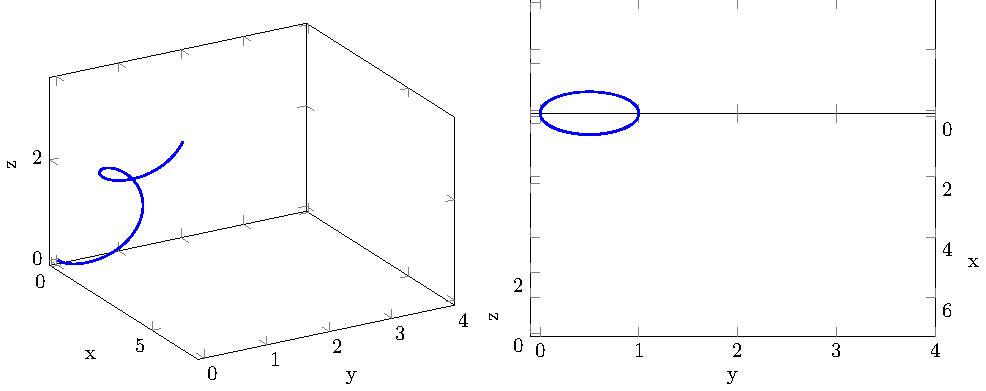
\includegraphics{Tikz1.pdf}
    \caption{Curva $\alpha$ com curvatura $\kappa_\alpha(t) = 1$ e torção $\tau_\alpha(t) = 1$, à esquerda com visualização geral e à direita ilustrando o círculo, caracterizado pela curvatura constante.}
\end{figure}

Um outro exemplo, um pouco mais divertido, traz uma curva cuja curvatura e torção não são constantes.

\begin{example}
    Encontrar a curva definida em $I = [0, 10]$ cuja curvatura é igual a $\kappa_\alpha(t) = t + 1$ e a torção é identificamente nula.
\end{example}

\noindent {\textbf{Solução:}} De modo análogo ao Exemplo \ref{exemplo_1}, precisaremos resolver um sistema de EDO's para encontrar a curva. Para essa curva, o sistema correspondente é o que pode ser visto em \ref{sistema_exemplo_2}.
\begin{equation}
    \label{sistema_exemplo_2}
    \left\{
        \begin{array}{rl}
            T'(t) & = (t + 1)N(t) \\
            N'(t) & = - (t + 1)T(t) + 0\cdot B(t) \\
            B'(t) & = - 0\cdot N(t)
        \end{array}
    \right.
\end{equation}

A resolução do sistema é uma atividade mais mecânica e, como já desenvolvemos para o Exemplo \ref{exemplo_1}, optamos por omitir as contas. Como resultado teremos os seguintes vetores:
\[T(t) = \left(\cos{\dfrac{1}{2}t(t + 2)}, \sin{\dfrac{1}{2}t(t + 2)}, 0\right),\]
\[N(t) = \left(-\sin{\dfrac{1}{2}t(t + 2)}, \cos{\dfrac{1}{2}t(t + 2)}, 0\right),\]
\[B(t) = \left(0, 0, 1\right).\]

Consequentemente, nossa curva será dada por
\[\alpha(t) = \left(\int_0^t \cos{\dfrac{1}{2}u(u + 2)} ~du, \int_0^t \sin{\dfrac{1}{2}u(u + 2)} ~du, 0\right).\]

Note que essa é uma curva plana, resultado totalmente esperado pois, conforme visto em aula, uma curva com torção nula será plana.

\section{Animações}







\section{Conclusão}

Nesse trabalho vimos o Teorema Fundamental das Curvas Espaciais, o qual nos diz que uma curva no espaço é definida por uma função curvatura positiva e por uma função torção. Além disso, vimos como podemos obter uma curva possuindo tais funções, com o intuito de ilustrar o teorema. Por fim, apresentamos um programa que calcula, iterativamente, tais curvas.

\begin{thebibliography}{9}

\bibitem{cruz} Cruz, J. (2017). The Fundamental Theorem of Space Curves. doi: \url{http://math.uchicago.edu/~may/REU2017/REUPapers/Cruz.pdf}.

\bibitem{brockveld} Brockveld, L. de L. (2018). Um estudo sobre curvas no plano e no espaço. UFSC. doi: \url{https://repositorio.ufsc.br/bitstream/handle/123456789/188642/tcc_Leonardo.pdf}.

\bibitem{terng} Terng, CL. (2005). Math 162A Lecture notes on Curves and Surfaces, Part I. doi: \url{https://www.math.uci.edu/~cterng/162A_Lecture_Notes.pdf}.

\bibitem{picado} Picado, J. (2006). Notas de aula de Geometria Diferencial.

\bibitem{coda} Codá, F. (2015). Geometria Diferencial. IMPA. \url{https://www.youtube.com/watch?v=bZiAkM6ab08}.

\bibitem{lima} Lima, R. F. de. (2016). Introdução à Geometria Diferencial. SBM.

\end{thebibliography}

\end{document}